\documentclass{standalone}
\usepackage{tikz}
\usepackage{ctex,siunitx}
\setCJKmainfont{Noto Serif CJK SC}
\usepackage{tkz-euclide}
\usepackage{amsmath}
\usetikzlibrary{patterns, calc}
\usetikzlibrary {decorations.pathmorphing, decorations.pathreplacing, decorations.shapes,}
\begin{document}
\small
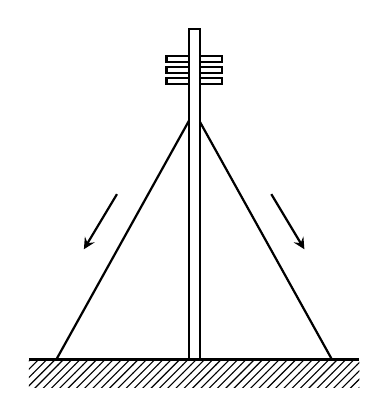
\begin{tikzpicture}[>=stealth, thick,scale=0.7]
  \fill [pattern = north east lines] (-3,-.5) rectangle (3,0);
  \draw(-3,0)--(3,0);
  \draw (0,4.5)--(-2.5,0);
  \draw (0,4.5)--(2.5,0);
  \foreach \x in{1,2,3}
  {
    \draw [fill=white] (-.5,4.8+\x*0.2) rectangle (.5,4.8+\x*0.2+.1);
  }
  \draw [fill=white] (-.1,0) rectangle (.1,6);
  \draw [->](-1.4,3)--(-2,2);
  \draw [->](1.4,3)--(2,2);
\end{tikzpicture}
\end{document}